% !TEX encoding = UTF-8 Unicode
\documentclass[a4paper]{article}

\usepackage{color}
\usepackage{url}
\usepackage[T2A]{fontenc} % enable Cyrillic fonts
\usepackage[utf8]{inputenc} % make weird characters work
\usepackage{graphicx}
\graphicspath{ {images/} }

\usepackage[english,serbian]{babel}
%\usepackage[english,serbianc]{babel} %ukljuciti babel sa ovim opcijama, umesto gornjim, ukoliko se koristi cirilica

\usepackage[unicode]{hyperref}
\hypersetup{colorlinks,citecolor=green,filecolor=green,linkcolor=blue,urlcolor=blue}

\usepackage{listings}

\usepackage{amsmath}
\usepackage{amsfonts}

% https://tex.stackexchange.com/questions/5223/command-for-argmin-or-argmax
\DeclareMathOperator*{\argmax}{argmax}

%\newtheorem{primer}{Пример}[section] %ćirilični primer
\newtheorem{primer}{Primer}[section]

\definecolor{mygreen}{rgb}{0,0.6,0}
\definecolor{mygray}{rgb}{0.5,0.5,0.5}
\definecolor{mymauve}{rgb}{0.58,0,0.82}

\lstset{ 
  backgroundcolor=\color{white},   % choose the background color; you must add \usepackage{color} or \usepackage{xcolor}; should come as last argument
  basicstyle=\scriptsize\ttfamily,        % the size of the fonts that are used for the code
  breakatwhitespace=false,         % sets if automatic breaks should only happen at whitespace
  breaklines=true,                 % sets automatic line breaking
  captionpos=b,                    % sets the caption-position to bottom
  commentstyle=\color{mygreen},    % comment style
  deletekeywords={...},            % if you want to delete keywords from the given language
  escapeinside={\%*}{*)},          % if you want to add LaTeX within your code
  extendedchars=true,              % lets you use non-ASCII characters; for 8-bits encodings only, does not work with UTF-8
  firstnumber=1000,                % start line enumeration with line 1000
  frame=single,	                   % adds a frame around the code
  keepspaces=true,                 % keeps spaces in text, useful for keeping indentation of code (possibly needs columns=flexible)
  keywordstyle=\color{blue},       % keyword style
  language=Python,                 % the language of the code
  morekeywords={*,...},            % if you want to add more keywords to the set
  numbers=left,                    % where to put the line-numbers; possible values are (none, left, right)
  numbersep=5pt,                   % how far the line-numbers are from the code
  numberstyle=\tiny\color{mygray}, % the style that is used for the line-numbers
  rulecolor=\color{black},         % if not set, the frame-color may be changed on line-breaks within not-black text (e.g. comments (green here))
  showspaces=false,                % show spaces everywhere adding particular underscores; it overrides 'showstringspaces'
  showstringspaces=false,          % underline spaces within strings only
  showtabs=false,                  % show tabs within strings adding particular underscores
  stepnumber=2,                    % the step between two line-numbers. If it's 1, each line will be numbered
  stringstyle=\color{mymauve},     % string literal style
  tabsize=2,	                   % sets default tabsize to 2 spaces
  title=\lstname                   % show the filename of files included with \lstinputlisting; also try caption instead of title
}

\begin{document}

\title{Automatsko prepoznavanje govora\\ \small{Seminarski rad u okviru kursa\\Metodologija stručnog i naučnog rada\\Matematički fakultet}}

\author{Vladimir Vuksanović, Aleksa Kojadinović, Lazar Čeliković\\vladevuksan99@gmail.com, drugog, trećeg autora}

%\date{9.~april 2015.}

\maketitle

\abstract{
  Prepoznavanje govora je jedan od osnovnih zadataka iz oblasti obrade prirodnog jezika (eng.~{\em natural laguage processing}). 
  Iako je prirodan za ljude, ovo je uvek bio težak zadatak za mašine.
  Tema ovog rada je da približi čitaoca zadatku automatskog prepoznavanja govora, problemima koji se javljaju i najznačajnijim arhitekturama ovih sistema.
  Biće reči o klasičnim, statističkim modelima kao i modernijim modelima potpuno zasnovanim na dubokim neuronskim mrežama.
  Poseban deo će biti izdvojen za opisivanje načina evaluacije modela i pregled performansi za neke od najznačajnijih.
}

\bigskip
\textbf{Ključne reči:} prepoznavanje govora

\tableofcontents

\newpage

\section{Uvod}
\label{sec:uvod}

Govor je za ljude najintuitivniji i najprirodniji način komunikacije. 
Zbog toga je u toku razvoja računarskih sistema, nastala ideja da isti vid komunikacije koristimo i za interakciju sa kompjuterima.
To bi znatno smanjilo potrebno predznanje za njihovo korišćenje i učnilio ih pristupačnijim većem broju ljudi. 
Najveća prepreka ovoj ideji do skoro je bilo kako sa velikom tačnosti prepoznati šta je korisnik rekao.
Taj postupak se naziva automatsko prepoznavanje govora.

\textbf{Automatsko prepoznavanje govora} (eng.~{\em Automatic Speech Recognition, ASR}) je proces pretvaranja zvučnog signala govora u odgovarajući niz reči pomoću kompjutera.
Neke od najznačajnijih primena ovih sistema danas su pametni lični asistenti (Google Assistant\footnote{https://assistant.google.com/}, Apple Siri\footnote{https://www.apple.com/siri/},\dots), transkripcija i pretraživanje audio sadržaja, automatsko titlovanje snimaka i pristupačnost.

Iako su istraživanja na ovu temu počela još sredinom dvadesetog veka, ovi sistemi su popularnost stekli tek u poslednjoj deceniji kada je uvođenje dubokih neuronskih mreža drastično povećalo njihove performanse.
Ta razlika je bila dovoljna da učini ove sisteme praktično primenljivim u odnosu na prethodne koji su bili nezgodni za upotrebu zbog velikog broja grešaka koje su pravili.
Prethodna decenija je videla i izjednačavanje sposobnosti računara i ljudi u prepoznavanju govora kada je kompanija Majkrosoft napravila sistem koji je ostvario iste rezultate kao ljudski eksperti na transkripciji Switchboard skupa podataka \cite{switchboard}.
% https://blogs.microsoft.com/ai/historic-achievement-microsoft-researchers-reach-human-parity-conversational-speech-recognition/
% https://www.microsoft.com/en-us/research/blog/microsoft-researchers-achieve-new-conversational-speech-recognition-milestone/
Za glavne uzroke ovog naglog poboljšanja se smatraju \cite{hannun2021history}:
\begin{enumerate}
  \item Sakupljanje ogromne količine tanskribovanih skupova podataka
  \item Nagli porast u performansama grafičkih procesorskih jedinica
  \item Poboljšanje algoritama za mašinsko učenje i arhitektura modela
\end{enumerate}

U nastavku ovog rada će prvo biti navedeni neki izazovi na koje se nailazi prilikom modelovanja sistema za prepoznavanja govora, zatim će biti opisan način rada dva najpopularnija modela: statistički i end-to-end i na kraju će biti predstavljen način za njihovu evaluaciju.

\section{Izazovi}
% https://www.youtube.com/watch?v=q67z7PTGRi8
Prepoznavanje govora je veoma težak zadatak zato što je potrebno da radi podjednako dobro u veoma različitim uslovima.
Neki od najvećih izazova su:
\begin{itemize}
  \item \textbf{Mala količina podataka za trening} --- 
  Za ostvarivanje dobrih rezultata potrebno je sakupiti više stotina ili čak hiljada sati labeliranih zvučnih snimaka koji treba da sadrže više govornika razlicitog pola i starosti, koji govore različitim akcentima. 
  Dok u skorije vreme jeste nastao porast u količini dostupnih podataka, veliki problem još uvek predstavlja reprezentativnost različitih varijacija u govoru i nedostatak podataka za jezike sa manjim brojem govornika. 
  Zbog toga se istražuju alternativni načini za treniranje kao sto su samo-treniranje (eng.~{\em self-training}) \cite{baevski2020wav2vec}, iterativno treniranje \cite{park2020noisy} ili treniranje koristeći kompjuterski generisan glas \cite{hannun2014deep}. 
  U dodatku \ref{sec:skupovi} se može naći tabela sa pregledom nekih od najpopularnijih trening skupova na engleskom jeziku.
  
  \item \textbf{Stil govora} --- 
  Postoje različiti sistemi u zavisnosti od toga koji tip govora mogu da prepoznaju \cite{anusuya2010speech}. Tipovi govora poređani po težini propoznavanja su: 
  \begin{enumerate}
    \item Izolovane reči --- reči su razdvojene dugim periodima tišine
    \item Povezane reči --- reči su razdvojene kratkim pauzama
    \item Neprekidan govor --- uvežbani govor, čitanje ili diktiranje
    \item Spontani govor --- neuvežbani, prirodni govor 
  \end{enumerate}
  Prve implementacije prepoznavanja govora su radile na nivou izolovanih reči i koristile su se za prepoznavanje određenih komandi ili cifara.
  Danas se najviše truda ulaže u poboljšanje prepoznavanja neprekidnog i spontanog govora.

  \item \textbf{Karakteristike govornika} ---
  Svaki čovek ima različitu boju glasa i govori različitom brzinom. Čak i starost osobe i jačina govora bitno utiču na frekvenciju glasa.
  Poseban problem pravi postojanje različitih dijalekata i akcenata koji mogu da imaju potpuno različite načine za izgovaranje istih reči.
  Jedan način za rešavanje ovog problema je treniranje sistema na glasu govornika koji će ga koristiti.
  To su sistemi zavisni od korisnika (eng.~{\em speaker dependent}) i koriste se u slučajevima da samo jedna osoba treba da ih koristi.
  Sa druge strane postoje sistemi nezavisni od korisnika (eng.~{\em speaker independent}) koji treba da rade podjednako dobro za sve govornike.
  
  \item \textbf{Okruženje govornika} --- 
  Ovi sistemi će retko biti korišćeni u potpuno tihim prostorijama sa profesionalnom opremom za snimanje. Zbog toga treba da budu tolerantni na različite vrste pozadinske buke ili kvaliteta mikrofona. 
  Neke vrste šumova je moguće otkloniti analizom zvuka ili naprednijim metodama \cite{xu2015enhancement}, ali jedan od najvećih problema predstavlja postojanje drugih govornika u okolini.
  Te signale je često teško razlikovati od glasa primarnig govornika, i samim tim teško ukloniti.
  
  \item \textbf{Veličina rečnika} --- 
  Povećanje broja reči koje model može da prepozna takođe povećava njegovu složenost i otežava treniranje, ali se time dobija na tačnosti. 
  Zbog toga je potrebno naći dobar kompromis između veličine rečnika i složenosti modela. 
  U slučajevima kada je potrebno pouzdano prepoznati samo neki skup komandi koriste se mali rečnici i oni su često veoma pouzdani, ali za prepoznavanje opšteg govora današnji sistemi su trenirani na skupu od oko 50.000-100.000 reči.
\end{itemize}

\section{Statistički model}
\label{sec:statistical}

Dugo vremena statistički pristup je bio dominantan za sisteme za prepoznavanje govora.
Iako je u skorije vreme pao u senku modela zasnovanih na dubokim neuronskim mrežama opisanim u poglavlju \ref{sec:e2e} ovaj model je jos uvek u širokoj upotrebi i veoma vredan izučavanja.

% Large Vocabulary Continuous Speech Recognition a Review
Cilj ovih sistema je da pronađu najverovatniju transkripciju za zadati ulaz.
Formalno, neka je $\hat{W}$ optimalan niz reči za transkripciju nekog zvučnog signala $X$. Cilj je optimizovati formulu \cite{kamath2019nlp}:
\begin{equation*}
  \hat{W} = \argmax_{W} P(W|X)
\end{equation*}
primenom Bajesove formule to se može zapisati kao:
\begin{equation*}
  \hat{W} = \argmax_{W} \frac{P(X|W) P(W)}{P(X)}
\end{equation*}
a kako je $P(X)$ konstantno za konkretan ulaz, može da se eliminiše:
\begin{equation}
  \label{eq:stat1}
  \hat{W} = \argmax_{W} P(X|W) P(W)
\end{equation}
Ideja je umesto modeliranja $P(W|X)$ što je teško, odvojeno modelirati verovatnoće iz prethodne formule jer za to postoje bolje tehnike.

Najprirodniji način za računanje $P(X|W)$ bi bio da se $W$ podeli na reči i za svaku od njih računa verovatnoća da je izgovorena.
U nekim slučajevima, kao na primer kada treba prepoznati samo neki mali skup komandi, tada se i koristi ovaj pristup.
Problem nastaje u sistemima sa velikim vokabularom zato što postoji veliki broj varijacija u izgovoru reči, a trening skup sadrži možda par primera za svaku od njih što nije dovoljno da se dobro nauči njeno prepoznavanje.
Dakle, umesto na reči potrebna je finija podela i za tu potrebu se koriste foneme.
\textbf{Foneme} su najmanje jezičke jedinice na osnovu kojih mogu da se razlikuju značenja većih jedinica.
One postoje samo kao apstraktna ideja, a njihova fizicka realizacija se zove glas.

Ako je $S$ niz fonema, $P(X|W)$ iz formule \ref{eq:stat1} se razlaže i dobija se:
\begin{equation*}
  \hat{W} = \argmax_{W} \sum_{S} P(X,S|W) P(W)
\end{equation*}
što se može aproksimirati kao:
\begin{equation}
  \label{eq:stat2}
  \hat{W} \approx \argmax_{W,S} P(X|S) P(S|W) P(W)
\end{equation}
Veličine iz prethodne formule imaju svoja imena na osnovu komponente koja ih računa:
$P(X|S)$ se naziva \textbf{akusticki model} (eng.~{\em acoustic model}), 
$P(S|W)$ je \textbf{model izgovora} (eng.~{\em pronunciation model}),
a $P(W)$ se zove \textbf{jezički model} (eng.~{\em language model})\footnote{Neka literatura $P(X|W)$ naziva akustičkim modelom, a model izgovora tretira kao njegov deo. U ovom radu će biti podrazumevano da su oni odvojeni modeli.}.

% https://www.idiap.ch/software/bob/docs/bob/bob.kaldi/stable/_images/ASR.png
Na slici \ref{fig:statistical_model} je prikazana cela struktura statističkog modela od zvučnog signala do transkripcije:
\begin{figure}[h!]
  \begin{center}
    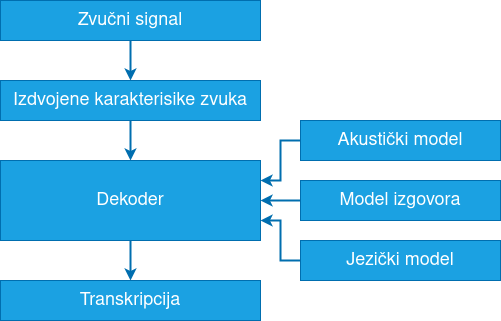
\includegraphics[scale=0.5]{statistical_model.png}
  \end{center}
  \caption{Statisticki model}
  \label{fig:statistical_model}
\end{figure}

U nastavku će biti opisana svaka od prikazanih komponenti, njena uloga i način rada.

\subsection{Obrada zvučnog signala}
\label{sec:obrada}
Sirovi zvučni signal je veoma nepogodan za korišćenje zato što sadrži veliku količinu nebitnih informacija i šuma.
Zbog toga se, pre prosleđivanja akustičkom modelu, signal prvo obrađuje tako da ostanu samo ključne karakteristike i smanji šum i veličina reprezentacije.

Signal se deli na kratke segmente koji se zovu \textbf{okviri} (eng.~{\em frame}).
Svaki od njih je fiksne dužine (obično 10-30 milisekundi) sa kratkim preklapanjem sa susednim okvirima radi smanjenja naglih promena prilikom prelaska iz jednog u drugi.
Pretpostavka je da je u svakom okviru glas konstantan, to jest da se glasovi mogu menjati samo prelaskom iz jednog okvira u drugi.
Na svaki od tih novodobijenih delova se zatim primenjuje neka vrsta spektralne analize najčešće zasnovana na Furijeovoj transformaciji kojom se izdvajaju samo njegove najbitnije karakteristike.
Tačna reprezentacija koja se koristi varira u zavisnosti od modela, ali jedna od najpopularnijih je \textbf{MFCC} (Mel-Frequency Cepstral Coefficients) \cite{dave2013feature} zasnovana na Mel skali koja oponaša ljudski slušni sistem.
Ovako obrađen signal se prosleđuje akustičkom modelu.

\subsection{Akustički model}
% https://cs229.stanford.edu/section/cs229-hmm.pdf
% https://www.cs.cmu.edu/~roni/10601-slides/hmm-for-asr-whw.pdf
Akustički model je zadužen da pretvori obrađeni zvučni signal u niz fonema. 
Ovaj zadatak predstavlja idealan slučaj za primenu skrivenih Markovljevih modela \cite{rabiner1989hmm}.

\textbf{Skriveni Markovljev model} (eng.~{\em hidden Markov model}) je dinamički sistem kojeg karakteriše sledeće:
\begin{enumerate}
  \item $N$ skrivenih stanja $S = \{S_1, S_2, \dots, S_N\}$ pri cemu $q_t$ označava stanje u trenutku $t$
  \item $M$ obzervacionih simbola $V = \{V_1, V_2, \dots, V_M\}$ pri cemu $o_t$ označava obzervaciju u trenutku $t$
  \item Raspodela verovatnoća promene stanja predstavljena matricom $A=\{a_{ij}\}$ dimenzije $N \times N$ gde važi: $$a_{ij} = P(q_{t+1} = S_j | q_{t} = S_i) \quad 1 \leq i,j \leq N$$
  \item Raspodela verovatnoća obzervacionih simbola iz stanja $j$ predstavljena matricom $B=\{b_j(k)\}$ dimenzije $N \times M$ gde važi: $$b_j(k) = P(o_t = V_k | q_t = S_j) \quad 1 \leq j \leq N, 1 \leq k \leq M$$
  \item Raspodela inicijalnog stanja $\pi=\{\pi_i\}$ gde važi: $$\pi_i = P(q_1 = S_i) \quad 1 \leq i \leq N$$
\end{enumerate}
Primer jednog modela je prikazan na slici \ref{fig:hmm}.

% https://www.researchgate.net/figure/State-transition-diagram-of-a-hidden-Markov-model_fig1_245563174
\begin{figure}[h!]
  \begin{center}
    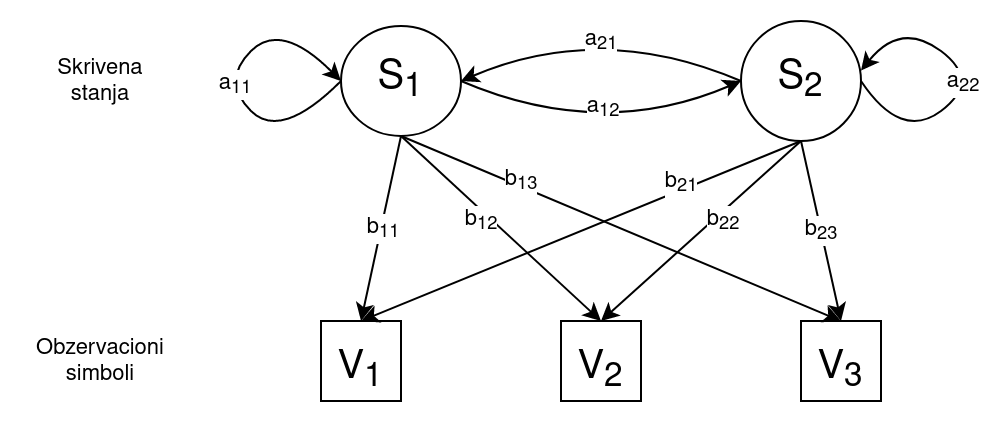
\includegraphics[scale=0.3]{hmm.png}
  \end{center}
  \caption{Primer skrivenog Markovljevog modela sa 2 skrivena stanja (krugovi) i 3 obzervaciona simbola (kvadrati)}
  \label{fig:hmm}
\end{figure}

Konkretno za prepoznavanje govora, skriveni Markovljevi modeli se koriste za opisivanje svake foneme.
Svaki od njih se sastoji od nekog zadatog broja stanja (obično 3 ili 5), a obzervacije su okviri zvučnog signala čije su verovatnoće predstavljene kao mešavina Gausovih raspodela.
Raspodele verovatnoća su dobijene treniranjem modela na skupu podataka.
Za svaku rečenicu iz trening skupa se konstruiše model spajanjem modela fonema u reči, pa reči u rečenicu.
Na njega se onda primeni Baum-Welch algoritam koji popravlja verovatnoće da više odgovaraju datim podacima.

Istrenirani model posle može da predvidi najverovatniji niz fonema (stanja) za datu obzervaciju koristeći Vetrebi algoritam za pretragu.

\subsection{Model izgovora}
U prethodnoj sekciji je rečeno da se prilikom treniranja modeli fonema spajaju u modele reči, ali nije objašnjeno tačno kako se to radi.
To je baš zadatak modela izgovora.
On je u suštini veliki rečnik koji za svaku reč čuva niz fonema kako se ona izgovara.
Ako postoji više varijacija izgovora, one se smatraju kao ražlicite stavke u rečniku.
Sada konstrukcija modela reči postaje trivijalna, samo se pronađe njen izgovor u rečniku i nadovežu odgovarajuci modeli fonema.
Ukoliko se reč ne nalazi u rečniku, sistem za prepoznavanje govora neće biti u stanju da je prepozna.

Prirodno sledeće pitanje je kako se određuju ova preslikavanja. 
Ovo je zapravo jedan od najtežih zadataka za modeliranje zato što se on ne uči na skupu podataka nego ga konstruišu eksperti iz tog domena.
Za svaku reč, neko je morao da zapiše na koji način se izgovara uzimajući u obzir da potencijalno postoji više izgovora.
Sa obzirom da današnji sistemi razlikuju oko 100.000 reči, ovo nimalo nije lak posao.

\subsection{Jezički model}
Povratkom na formulu \ref{eq:stat2}, jezički model dodeljuje verovatnoću pojavljivanja $P(W)$ svakoj mogućoj sekvenci reči $W$.
Ovde se uzima u obzir relativna učestalost reči, verovatnoća da se reči nađu jedna za drugom, i mogu da se vrše dodatne sintaksne i semantičke provere.
Postoje rečenice koje zvuče slično ali nemaju sve semantičko znacenje.
Tada se od njih bira ona koja ima najviše smisla.
% primer

Kako $P(W)$ ne zavisi od zvučnog signala, može se odvojeno trenirati na samo tekstualnom skupu podataka kojih postoji dosta više i imaju veći broj primera od skupova sa transkribovanim snimcima.
U nekim slučajevima trenirana raspodela se može promeniti u zavisnosti od korisnika (npr. pametni lični asistenti prepoznaju kontakte na korisnikovom telefonu).

Najčešći vid implementacije ovog modela je pomoću n-grama.
Neka se transkripcija $W$ razdvaja na reči $W = \{w_1, w_2, \dots, w_m\}$ i neka je $n$ dužina n-grama.
To znači da pri računanju verovatnoće pojavljivanja neke reči u obzir uzimamo samo $n-1$ njenih prethodnika.
Tada se $P(W)$ može predstaviti kao:
\begin{equation*}
  P(W) = \prod_{i=1}^{m} P(w_i | w_1,\dots,w_{i-1}) = \prod_{i=1}^{m} P(w_i | w_{i-n+1},\dots,w_{i-1})
\end{equation*}
Ako $C(x)$ označava broj pojavljivanja sekvence $x$ u trening skupu, verovatnoća da je $w_i$ sledeća reč se može proceniti kao:
\begin{equation*}
  P(w_i | w_{i-n+1},\dots,w_{i-1}) = \frac{C(w_{i-n+1},\dots,w_i)}{C(w_{i-n+1},\dots,w_{i-1})}
\end{equation*}
Radi jednostavnije implementacije na početak $W$ se dodaje $n-1$ "prazna" reč.

Veliki problem sa ovim modelom je što onemogućava predviđanje n-grama koji nisu prethodno viđeni u trening skupu jer bi im bila dodeljena verovatnoća 0.
Čak i za male vrednosti $n$ ovo nije nerealna situacija.
Kao kompenzacija za to moguće je umesto fiksnog, koristiti promenljivo $n$ koje bi krenulo od neke zadate vrednosti i smanjivalo se sve dok ne pronađe bar jedna instanca tog n-grama.
Onda je moguće direktno korisiti tu vrednost ili na neki način uračunati koliko se parametar smanjio pre nego što je n-gram pronađen.

\subsection{Dekodiranje}
\label{sec:dekodiranje}

Konstrukcijom svih prethodno opisanih komponenti i njihovim treniranjem, model je gotov i spreman za upotrebu.
Jedino što ostaje je pretražiti prostor dopustivih rečenica da se pronađe ona koja najviše odgovara glasovnom signalu.
U praksi, taj prostor je veoma veliki i njegova celokupna pretraga je eksponencijalne složenosti, stoga nije izvodljivo tražiti egzaktno rešenje.
Umesto toga se koristi heuristički, \textbf{beam search algoritam}.
Ideja je da se rešenje gradi iterativno i u svakom trenutku umesto testiranja svih mogućih puteva gramzivo se bira samo $b$ najverovatnijih.
Parametar $b$ se određuje tako da balansira veličinu prostora za pretraživanje i vreme potrebno za njegov obilazak.
Dakle, algoritam počinje od niza sa jednom praznom rečenicom.
Jedan korak se sastoji od produživanja svakog elementa iz niza svim mogućim rečima i brisanja svih osim $b$ najverovatnijih.
Ta verovatnoća se jednostavno računa množenjem verovatnoće nove reči sa verovatnoćom rečenice koja je dopunjena.
Ovaj postupak se ponavlja sve do kraja svih rečenica iz niza kada se najverovatnija od njih proglašava za konačnu transkripciju govora.

\section{End-to-end model}
\label{sec:e2e}

End-to-end model je ceo zasnovan na dubokim neuronskim mrežama.
Za razliku od statističkog modela koji proces prepoznavanja govora deli u više složenijih celina, end-to-end model je po strukturi prostiji.
Umesto razdvajanja formule \ref{eq:stat1} pomoću Bajesovog pravila, on direktno računa verovatnoću $P(W|X)$, to jest
bave se direktnim prevođenjem ulaznog zvučnog signala u niz grafema, karatera ili reči.
To donosi velike prednosti, naime: više nije potreban ekspert za jezik nego se sve uči iz podataka, treniranje postaje lakše zbog jednostavnije strukture i performanse postaju bolje zato što se optimizuje samo jedna vrednost.
Sa druge strane, pošto model treba sam sve da nauči, potrebna je veća količina podataka nego ako se koristi statistički model.

Glavni problem ovim modelima je kako odrediti kom delu zvuka odgovara deo transkripcije.
To je posao koji su u statističkom pristupu radili skriveni Markovljevi modeli.
U odnosu na način rešavanja ovog problema razlikuju se \textbf{CTC} \cite{graves2006ctc} i \textbf{modeli zasnovani na pažnji} (eng.~{\em attention based models}) \cite{chorowski2015attentionbased}.

\subsection{CTC model}
\label{sec:ctc}

CTC (Connectionist Temporal Classification) rešava problem poravnanja zvuka i teksta tako što tretira izlaz iz mreže kao raspodelu verovatnoća za svaku labelu ili blanko karakter.
Ideja iza uvođenja ovog karaktera je da se pomoću njega vrši poravnanje sa zvukom, ali da se on ignoriše prilikom predviđanja labela.

Neka je ulazni zvuk podeljen na segmente jednakih dužina, gde je svaki od njih obrađen u vektor realnih brojeva dužine $m$\footnote{Ovo može da bude MFCC kao u poglavlju \ref{sec:obrada}, ali je češće nešto jednostavnije} i neka je $L$ konačna azbuka labela (oznaka).
Cilj je napraviti preslikavanje $h$ koje slika proizvoljan zvučni signal u niz labela:
\begin{equation}
\label{eq:pres1}
h: (\mathbb{R}^m)^* \rightarrow L^* 
\end{equation}
U praksi je broj vremenskih trenutaka fiksiran na neku vrednost $T$.
Iako je broj trenutaka fiksiran za zvučne signale, nizovi labela ne moraju biti iste dužine za svaku ulaznu instancu, stoga jednu trening instancu predstavlja par $(\textbf{x}, \textbf{z})$ gde je $\textbf{z}$ vektor labela dužine najvise $T$.

Ako $O$ označava test skup, tada se funkcija greške definiše na sledeći način:
\begin{equation}
\label{eq:LER}
LER(h, O) = \frac{1}{|O|}\sum_{(\textbf{x}, \textbf{z}) \in O}\frac{ED(h(\textbf{x}), \textbf{z})}{\textbf{|z|}}
\end{equation}
gde $ED$ predstavlja edit rastojanje\footnote{minimalni broj izmena koji dovodi jedan niz karaktera do drugog, pri čemu dozvoljene izmene podrazumevaju brisanje, zamenu i umetanje karaktera}. Prethodna mera naziva se stopa greske labela (eng.~{\em label error rate - LER}).
Formula \ref{eq:LER} je prirodna ocena greške za probleme koji za cilj imaju minimizaciju greške prevođenja.

Model se implementira kao rekurentna neuronska mreža koja za svaki od $T$ trenutaka ima $m$ ulaza, a izlaz je softmax sloj dimenzije $|L'|$, gde je $L'$ azbuka proširena blanko karakterom, $L' = L \cup \{\epsilon\}$.
Svaki izlaz se interpretira kao raspodela verovatnoća za pojavljivanje odgovarajuće labele iz $L'$ u tom vremenskom trenutku.
Neformalno rečeno, prolaskom kroz izlaze u svakom od $T$ trenutaka dobija se putanja $\pi \in (L')^T$ koja predstavlja jedan mogući odabir labela.
Ako $y_{\pi_t}^t$ predstavlja softmax vrednost u trenutku $t$ oznake $\pi_t$, tada je verovatnoća odabira kompletne putanje:
\begin{equation*}
  P(\pi|\textbf{x}) = \prod_{t=1}^Ty_{\pi_t}^t
\end{equation*}

U praksi, zvuk je segmentovan na veoma sitne vremenske intervale (oko 10ms), stoga je pojava blanko ili dupliciranih oznaka veoma česta. 
Iz tog razloga se uvodi preslikavanje $\mathcal{B}$ čija je uloga prečišćavanje nizova labela uklanjanjem blanko oznaka i susednih duplikata.
\begin{equation*}
  \mathcal{B}: (L')^T \rightarrow L^U, U \leq T
\end{equation*}
Kako za jednu prečišćenu putanju $l$ može postojati više mogućih izvornih putanja, verovatnoća njenog odabira jednaka je sumi po svim izvornim putanjama.
\begin{equation}
\label{eq:beta}
  P(l | x) = \sum_{\pi \in \mathcal{B}^{-1}(l)} p(\pi | \textbf{x})
\end{equation}

Imajući u vidu sve prethodno navedeno, zadatak preslikavanja $h$ je odabir najverovatnije prečišćene putanje za dati ulaz.
\begin{equation}
\label{eq:h_x}
  h(x) = \argmax_{l \in L^U} P(l | \textbf{x})
\end{equation}
Ovo je moguće na više načina.
Najjednostavniji, ali neoptimalan, jeste pohlepni odabir najbolje oznake za svaki vremenski trenutak ponaosob, ali postoje i drugi algoritmi koji daju bolje rezultate.

% RNN-T

\subsection{Modeli zasnovani na paznji}

Za razliku od CTC modela, ovi modeli se oslanjaju na \textbf{mehanizmam pažnje} (eng.~{\em attention mechanism}) za poravnjanje teksta sa zvukom i odbacuju problematičnu pretpostavku o nezavisnosti zvučnih segmenata na kojoj se CTC zasniva.
Ova grupu modela će biti predstavljena na primeru LAS (eng.~{\em Listen, Attend and Spell}) modela \cite{chan2015las}. 

Glavne komponente ovog modela su \textbf{slušalac} (eng.~{\em listener}) i \textbf{speler} (eng.~{\em speller}).
Okvirno gledano, uloga slušaoca jeste da transformiše ulazni signal u karakteristike višeg nivoa, koje se prosleđuju speler komponenti da proizvede konačan niz karaktera. 

Slično kao u poglavlju \ref{sec:ctc}, neka je $\textbf{x}$ = $(x_1,  x_2,  ...,  x_T)$ ulazni signal, a $\textbf{y}$ niz mogućih izlaznih karaktera (uključujući razmak, tačku, zarez, apostrof) i specijalnih karaktera (početak i kraj rečenice i nepoznat simbol).
Cilj je modelovati $\textbf{y}$ kao uslovnu raspodelu u zavisnosti od ulaznog signala $\textbf{x}$ i prethodnih izlaza $y_j,  j \in (1,  i-1)$
\begin{equation}
  \label{eq:chain}
  P(y | x) = \prod_i P(y_i | x, y_j, j < i)
\end{equation}

Skušalac je rekurentna neuronska mreža piramidalne strukture čiji zadatak je da napravi reprezentaciju zvuka višeg nivoa. 
Kao što se može primetiti na slici \ref{fig:listener_model}, broj neurona se polovi u svakom sloju do izlaznog.
Ova osobina omogućava smanjenje složenosti izračunavanja, što je veoma poželjno u slučaju kada je dužina zvučnog segmenta mala.
\begin{figure}[h!]
  \begin{center}
    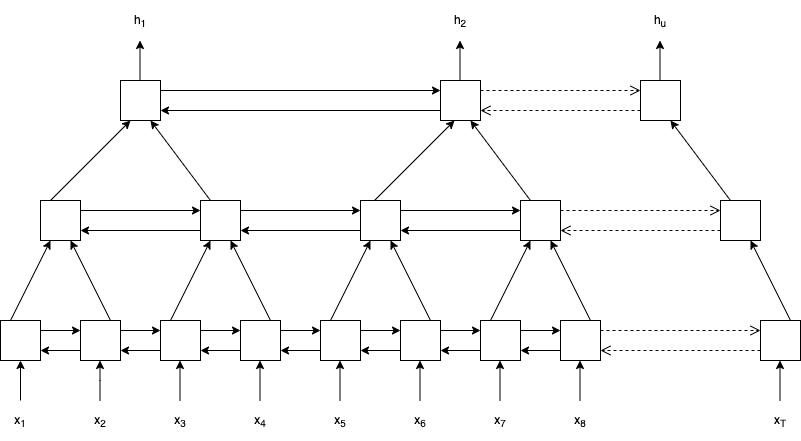
\includegraphics[scale=0.3]{listener.png}
  \end{center}
  \caption{Listener neuronska mreža}
  \label{fig:listener_model}
\end{figure}

Speler je takođe rekurentna neuronska mreža.
Kao sto je već pomenuto, verovatnoća odabira svakog karaktera zavisi od odabira svih prethodnih.
Na izlaz $y_i$ utiče stanje $s_i$ i kontekst $c_i$.
Stanje se računa rekurentno na osnovu prethodnog stanja, izlaza i konteksta, a kontekst se izračunava korišćenjem standardnog mehanizma pažnje.
Intuitivno, kontekst prikuplja relevantno znanje o okolnim zvučnim segmentima potrebnim za predikciju narednog karaktera, na taj način određujući koliko znanje o okolini utiče na znanje o trenutnom karakteru.
Struktura ove mreže je prikazana na slici \ref{fig:speller_model}. 
%  \begin{equation}
% \label{eq:state}
% s_i = RNN (s_{i-1},  y_{i-1},  c_{i-1})
% \end{equation}
\begin{figure}[h!]
  \begin{center}
    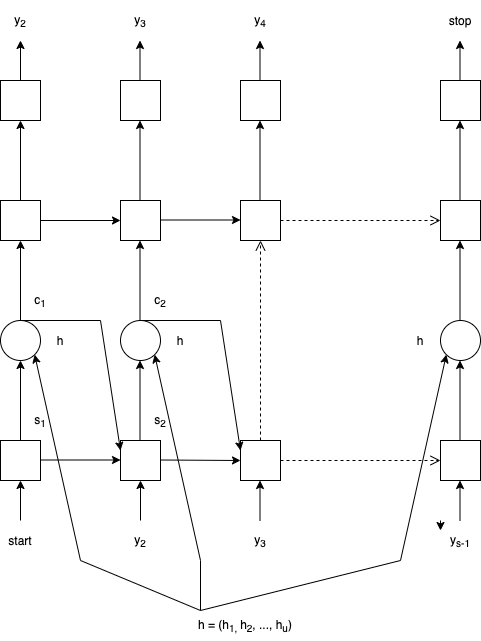
\includegraphics[scale=0.3]{speller.png}
  \end{center}
  \caption{Speller neuronska mreža}
  \label{fig:speller_model}
\end{figure}

Treniranje se sprovodi određivanjem parametara koji maksimizuju sumu logaritama uslovnih verovatnoća za svaki karakter.
\begin{equation}
  \label{eq:max}
  \max_{\theta} \sum_i \log P(y_i | \textbf{x}, \bar{y}_j, j < i; \theta)
\end{equation}
gde je $\bar{y_j}$ objektivna vrednost karaktera $j$.

Konačno dekodiranje se vrši heuristički, kao u poglavlju \ref{sec:dekodiranje} po prostoru pretrage određenom raspodelama verovatnoća iz svakog koraka speler rekurentne mreže.

\section{Metrike za evaluaciju}
Standardna mera za procenu kvaliteta sistema za prepoznavanje govora je \textbf{stopa pogrešnih reci} (eng.~{\em word error rate, WER}).
Za njeno izračunavanje potrebno je da imamo generisan tekst koji evaluiramo i tačnu transkripciju kao referencu.
Formula je izvedena normalizacijom Levenštajnovog rastojanja i izgelda ovako:
\begin{equation*}
  WER = \frac{I + D + S}{N}
\end{equation*}
gde je:
\begin{itemize}
  \item $I$ broj umetnutih reči
  \item $D$ broj obrisanih reči
  \item $S$ broj zamenjenih reči
  \item $N$ ukupan broj reči u referenci
\end{itemize}
Minimalna vrednost koju može da ima je 0, dok maksimalna vrednost može da bude preko 1 (npr. izgovorena je jedna reč a prepoznate dve).
Stopa pogrešnih reči se efikasno računa dinamičkim programiranjem, pomoću Vagner-Fišerovog algoritma (eng.~{\em Wagner-Fischer algorithm}). % čiji pseudokod se može naći u dodatku

Cilj sistema za prepoznavanje govora je da minimizuje ovu vrednost.

\section{Zaključak}
\label{sec:zakljucak}

Kroz ovaj rad predstavljeni su osnovni pojmovi i najznačajniji modeli za automatsko prepoznavanje govora.
Uprkos tome što su end-to-end modeli dosta korišćeniji u praksi zbog generalno boljih performansi, statistički modeli su i dalje široko rasprostranjeni i još uvek su predmet brojnih istraživanja.

Ovaj rad je bio samo uvod u automatsko prepoznavanje govora i čitalac se poziva da samostalno nastavi istraživanje na ovu temu.
Radovi iz literature sadrže više informacija o konceptima i implementaciji pomenutih modela koje su bile izvan opsega ovog rada i predstavljaju dobar početak za dalje istraživanje.

% \section{Osnovna uputstva}
% Vaš seminarski rad mora da sadrži najmanje jednu \textbf{sliku}, najmanje jednu \textbf{tabelu} i najmanje \textbf{sedam referenci} u spisku literature. Najmanje jedna slika treba da bude originalna i da predstavlja neke podatke koje ste Vi osmislili da treba da prezentujete u svom radu. Isto važi i za najmanje jednu tabelu. 	Od referenci, neophodno je imati bar jednu \textbf{knjigu}, bar jedan \textbf{naučni članak} iz odgovarajućeg časopisa i bar jednu adekvatnu \textbf{veb adresu}. 
% \textbf{Dužina seminarskog rada treba da bude od 10 do 12 strana.} Svako prekoračenje ili potkoračenje biće kažnjeno sa odgovarajućim brojem poena. Eventualno, nakon strane 12, može se javiti samo tekst poglavlja \textbf{Dodatak} koji sadrži nekakav dodatni k\^{o}d, ali je svakako potrebno da rad može da se pročita i razume i bez čitanja tog dodatka. 

\addcontentsline{toc}{section}{Literatura}
\appendix
\bibliography{seminarski} 
% \bibliographystyle{plain}
\bibliographystyle{ieeetr}

\appendix

% dodatak: pregled skupa podataka za trening
% https://github.com/double22a/speech_dataset
% CommonVoice - https://commonvoice.mozilla.org/en/datasets
% TIMIT - https://catalog.ldc.upenn.edu/LDC93S1 https://github.com/philipperemy/timit
% Switchboard 1 - https://catalog.ldc.upenn.edu/LDC97S62 https://www.kaggle.com/nltkdata/switchboard
% LibriSpeech - https://openslr.org/12/ https://www.danielpovey.com/files/2015_icassp_librispeech.pdf
% GigaSpeech - 
% WSJ1 - https://catalog.ldc.upenn.edu/LDC94S13A
% Fisher
\section{Dodatak: Pregled skupova podataka}
\label{sec:skupovi}

\begin{table}[h!]
\begin{center}
  \caption{Pregled nekih od najznačajnijih skupova podataka transkribovanog govora.}
  \begin{tabular}{|c|c|c|c|}
    \hline
    Naziv skupa   & Dužina (sati) & Broj govornika & Nivo transkripcije \\
    \hline
    TIMIT         & 5,4           & 630            & foneme, reči       \\ 
    Switchboard-1 & 260           & 543            & reči               \\ 
    LibriSpeech   & 982,1         & 1166           & reči               \\ 
    CommonVoice   & 2015          & 75.879         & reči               \\
    GigaSpeech    & 10.000        & nepoznato      & reči               \\
    VoxPopuli     & 543           & 413.581        & reči               \\
    % Naziv skupa   & Duzina (sati) & Broj recenica & Broj govornika & Nivo transkripcije \\
    % \hline
    % TIMIT         & 5,4           & 6300          & 630            & foneme, reci       \\ 
    % Switchboard-1 & 260           & 2438 konv     & 543            & reci               \\ 
    % LibriSpeech   & 1000 (982.1)  & nepoznato     & 1166           & reci               \\ 
    % CommonVoice   & 2015          & nepoznato     & 75.879         & reci               \\
    % GigaSpeech    & 10.000        & ?             & nepoznato      & reci               \\
    % VoxPopuli     & 543           & 1313          & 413.581        & reci               \\
    % WSJ 1         & 80            & nepoznato     & nepoznato      & reci               \\
    \hline
  \end{tabular}
  % \label{tab:tabela1}
\end{center}
\end{table}

\end{document}

